% Created 2025-03-28 Fri 21:14
% Intended LaTeX compiler: pdflatex
\documentclass[conference]{IEEEtran}
\usepackage[utf8]{inputenc}
\usepackage[T1]{fontenc}
\usepackage{graphicx}
\usepackage{longtable}
\usepackage{wrapfig}
\usepackage{rotating}
\usepackage[normalem]{ulem}
\usepackage{amsmath}
\usepackage{amssymb}
\usepackage{capt-of}
\usepackage{hyperref}
\IEEEoverridecommandlockouts
\usepackage{cite}
\usepackage{amsmath,amssymb,amsfonts}
\usepackage{algorithmic}
\usepackage{graphicx}
\usepackage{textcomp}
\usepackage{xcolor}
\usepackage[hidelinks]{hyperref}
\usepackage{hanging} %% for IEEE-style hanging indent in References section.
\input{/home/praaneshnair/.config/doom/def.tex}
\input{/home/praaneshnair/.config/doom/author.tex}
\graphicspath{ {.} }
\date{}
\title{Prediction of Ground Motion using Data on Seismic Waves}
\hypersetup{
 pdfauthor={Praanesh Balakrishnan Nair},
 pdftitle={Prediction of Ground Motion using Data on Seismic Waves},
 pdfkeywords={},
 pdfsubject={},
 pdfcreator={Emacs 29.4 (Org mode 9.7.19)}, 
 pdflang={English}}
\begin{document}

\maketitle
\begin{abstract}
This paper presents a methodology for analyzing seismic data from significant
earthquakes using the ObsPy Python library. Our dataset encompasses four major
seismic events: the 2011 Tohoku earthquake (Japan), the 2010 Chile earthquake,
the 2016 Kumamoto earthquake (Japan), and the 2015 Nepal earthquake. The utility
of the processed data is demonstrated by applying the Short-Term
Average/Long-Term Average (STA/LTA) algorithm to the mean-subtracted waveforms
to automatically identify the arrival of P-Waves and S-Waves. A k-Nearest
Neighbours (kNN) regression model was used to predict the peak ground
acceleration (PGA) and Arias intensity for each event.


\end{abstract}


\begin{IEEEkeywords}

Seismic Waves, Instrument Response, Ground Acceleration, Arias Intensity

\end{IEEEkeywords}
\section{Introduction}
\label{sec:orgc9e60f9}
The analysis of seismic data provides crucial insights into earthquake dynamics
and Earth's subsurface structure. Various seismic waveform data from several
significant earthquakes were processed and analyzed by investigating the
relationship between maximum amplitude and distance to the event. This was done
by extracting features, using matrix operations and similarity measures. We
focus on four major seismic events: the 2011 Tohoku earthquake (Japan), the 2010
Chile earthquake, the 2016 Kumamoto earthquake (Japan), and the 2015 Nepal
earthquake. This approach facilitates access to a large volume of data from
diverse sources.
\section{Literature Survey}
\label{sec:orgfba83d2}
Seismic signal processing and analysis have garnered significant attention in
recent years, with various machine learning methodologies being employed for
classification, event detection, and predictive modeling. This section reviews
key contributions in the field, highlighting different approaches and techniques
applied to seismic data analysis.


Li et al. \cite{b1} investigated seismic data
classification using supervised machine learning techniques. Their study focused
on extracting features such as spectral content, amplitude variations, and
waveform characteristics. They evaluated the performance of multiple machine
learning models, including Support Vector Machines (SVM), Decision Trees, and
Neural Networks, which were trained on labeled seismic event datasets to assess
classification accuracy.


Ramirez and Meyer \cite{b2} explored seismic phase
classification through manifold learning techniques. Their approach involved
mapping high-dimensional seismic data onto a lower-dimensional manifold using
Laplacian Eigenmaps, improving classification performance by preserving local
waveform structures. Their method demonstrated enhanced differentiation between
P-waves and S-waves using nearest-neighbor-based classifiers in the transformed
space.


Chakraborty et al. \cite{b3} employed statistical feature extraction
techniques for micro-seismic event detection. The extracted features included
peak amplitude, energy, zero-crossing rate, and entropy. Machine learning models
such as Random Forest, SVM, and k-Nearest Neighbors (KNN) were applied to
classify seismic events, distinguishing natural seismic activity from noise with
improved accuracy.


Shu et al. \cite{b4} conducted a comprehensive survey on
machine learning applications in microseismic signal recognition and
classification. They categorized methodologies into three major groups:
feature-based models utilizing statistical descriptors, deep learning models
such as Convolutional Neural Networks (CNNs) and Recurrent Neural Networks
(RNNs), and hybrid techniques that integrate statistical feature extraction with
deep learning frameworks. Additionally, their survey highlighted key challenges
and potential advancements in the domain.


Varshney et al. \cite{b5} developed a
machine learning-based earthquake monitoring system leveraging real-time seismic
data streams. Their approach involved preprocessing seismic data using Fourier
and Wavelet Transforms before training classification models, such as Decision
Trees and Neural Networks, to detect and monitor earthquake events dynamically.


Chin et al. \cite{b6} enhanced earthquake detection accuracy by implementing a
hybrid deep learning model integrating CNNs and Long Short-Term Memory (LSTM)
networks. Their framework, trained on labeled seismic waveform datasets,
incorporated data augmentation techniques to improve model robustness. The
proposed system demonstrated superior detection performance compared to
traditional signal processing methods.


Shimshoni and Intrator \cite{b7} applied
ensemble learning techniques for seismic signal classification. Their work
utilized bagging and boosting strategies to enhance classification accuracy,
demonstrating that ensemble-based neural network approaches could improve
differentiation between seismic events.


Agliz and Atmani \cite{b8} employed
multi-layer perceptron (MLP) neural networks for seismic signal classification.
Their methodology involved extracting both frequency-domain and time-domain
features from seismic waveforms, which were subsequently used as input to the
neural network for classification and training.


Akhouayri et al. \cite{b9}
introduced a fuzzy expert system for automatic seismic signal classification.
Their method defined fuzzy sets based on key signal parameters such as
amplitude, frequency content, and duration, allowing for a more flexible and
interpretable classification framework compared to traditional rule-based
systems.


Curilem et al. \cite{b10} investigated the application of genetic
algorithms for optimizing neural network classifiers in the context of volcanic
seismic signal classification. Their findings demonstrated that evolutionary
computation techniques could enhance the performance of neural network models in
differentiating between various types of volcanic seismic events.
\section{Methodology}
\label{sec:org07ff969}
\subsection{Data Extraction}
\label{sec:orgb307f39}
The ObsPy Python library was used for obtaining seismic wave data within
20\(^{\circ}\) of the epicenter. The epicenter of the earthquake is at
37.52\(^{\circ}\) N and 143.04\(^{\circ}\) E, and the seismic activity was
observed from 60 seconds before the earthquake, to 600 seconds after the
earthquake. Using \texttt{obspy.mass\_downloader()}, waveform data was retrieved
in miniSEED format corresponding station metadata in StationXML format from
multiple data centers, including IRIS. The downloaded miniSEED files were
processed to extract key features for analysis. The seismic channels prioritized
are ``Horizontal North-South'' (HN), ``Broadband North-South'' (BN), ``Horizontal
Horizonal'' (HH) and ``Broadband Horizontal'' (BH).
\subsection{Data Preprocessing}
\label{sec:orgd9f8199}
Since different seismic instruments have different frequencies at which they are
most sensitive, the actual ground motion had to be isolated from the
instruments' behaviour. The raw waveform files were read and the instrument
response was removed, by using the right acceleration units and apply
pre-filtering of 0.01 Hz to 50 Hz to stabilize the data.
\subsection{Feature Extraction}
\label{sec:org1a5941c}
The features extracted were station latitude, longitude, station elevation,
distance from earthquake epicenter, Peak Ground Acceleration (PGA), Root Mean
Square (RMS) acceleration, Arias Intensity (measure of ground shaking severity),
Significant duration (time between 5-95\% cumulative energy), Predominant
frequency, Mean frequency, Spectral centroid and Energy distribution across
frequency bands.
\subsection{Training}
\label{sec:org92352c3}
After feature extraction, K-means algorithm was used to divide the data into 3
clusters, with the aim of identifying similar ground motion behaviour. This was
done after Principal Component Analysis (PCA) was used for reduction in
dimensionality.
\section{Results}
\label{sec:org226fbdd}
\subsection{K-Means Cluster Centers}
\label{sec:orga1dad42}
\begin{enumerate}
\item Cluster Center 1:
\begin{verbatim}
[  6.47288676e-02, -2.87186817e-02,
   1.95212192e-03,  6.10829146e-02,
  -2.02384596e-01, -2.13568800e-01,
  -1.85436858e-01,  1.14996457e-01,
  -1.48823025e-01, -1.40580481e-01,
  -1.40580481e-01, -1.29345298e-01,
  -1.68891165e-01, -1.24105794e-01  ]
\end{verbatim}

\item Cluster Center 2:
\begin{verbatim}
[ -1.83431692e+00,  2.03685872e+00,
  -7.60801964e-01, -3.04967223e+00,
   2.77600917e-01,  8.21964292e-01,
   7.40345250e-02, -8.40617717e-01,
  -3.47115600e-02,  2.73000124e-01,
   2.73000124e-01,  4.24253450e+00,
   5.10822384e+00,  1.59656704e-01  ]
\end{verbatim}

\item Cluster Center 3:
\begin{verbatim}
[ -2.11568015e-01, -9.06781101e-01,
   5.70831836e-01,  8.79265630e-01,
   5.12686448e+00,  4.97734930e+00,
   4.84507409e+00, -2.35440088e+00,
   3.96544584e+00,  3.49562898e+00,
   3.49562898e+00, -4.93935228e-02,
   2.88483144e-01,  3.15253417e+00  ]
\end{verbatim}
\end{enumerate}
\subsection{Evaluation Metrics}
\label{sec:orgbd00cab}
The clustering results were measured with the help of the evaluation metrics.
The Silhouette scores for each point at different values of \(k\) were
calculated. The formula used to calculate the Silhouette scores is given in
below equation.

\begin{equation}
S(i) = \frac{b(i) - a(i)}{\max(a(i), b(i))}
\end{equation}

where:
\begin{itemize}
\item \(a(i)\) is the average distance between point \(i\) and all other points in the same
\end{itemize}
cluster
\begin{itemize}
\item \(b(i)\) is the average distance between point \(i\) and all points
\end{itemize}
in the nearest different cluster.

\[ \]

When you have the total number of points (\(N\)), the overall Silhouette Score is simply the average of all the individual Silhouette Scores.

\begin{equation}
\text{Overall Silhouette Score} = \frac{1}{N} \sum_{i=1}^{N} S(i)
\end{equation}

        When \(k\) is a smaller number, the Silhouette Scores are better as
they are closer to 1. At larger values of \(k\), the data points appear to be
near the boundaries of the clusters.

\begin{figure}[htbp]
    \centering
    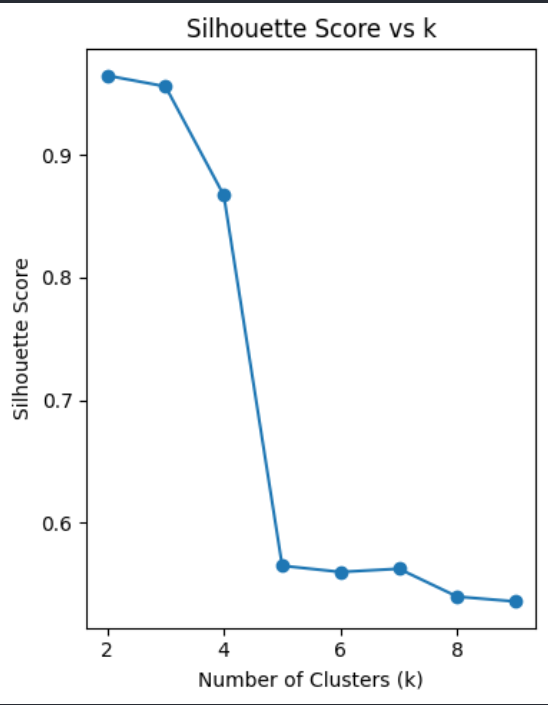
\includegraphics[width=\columnwidth]{silhouette_score.png}
    \caption{Silhouette Scores for Different Values of \(k\)}
    \label{fig:example}
\end{figure}

The Calinski-Harabasz scores measures the ratio of how seperated clusters are, to how tight each cluster is.

\begin{equation}
CH = \frac{\text{Tr}(B_k)}{\text{Tr}(W_k)} \times \frac{N - k}{k - 1}
\end{equation}

where:
\begin{itemize}
    \item \( B_k \) is the between-cluster dispersion matrix:
    \begin{equation}
    B_k = \sum_{i=1}^{k} n_i (\mu_i - \mu)(\mu_i - \mu)^T
    \end{equation}
    \item \( W_k \) is the within-cluster dispersion matrix:
    \begin{equation}
    W_k = \sum_{i=1}^{k} \sum_{x \in C_i} (x - \mu_i)(x - \mu_i)^T
    \end{equation}
    \item \( N \) is the total number of points.
    \item \( k \) is the number of clusters.
    \item \( n_i \) is the number of points in cluster \( i \).
    \item \( \mu_i \) is the centroid of cluster \( i \).
    \item \( \mu \) is the global centroid of all points.
\end{itemize}


\begin{figure}[htbp]
    \centering
    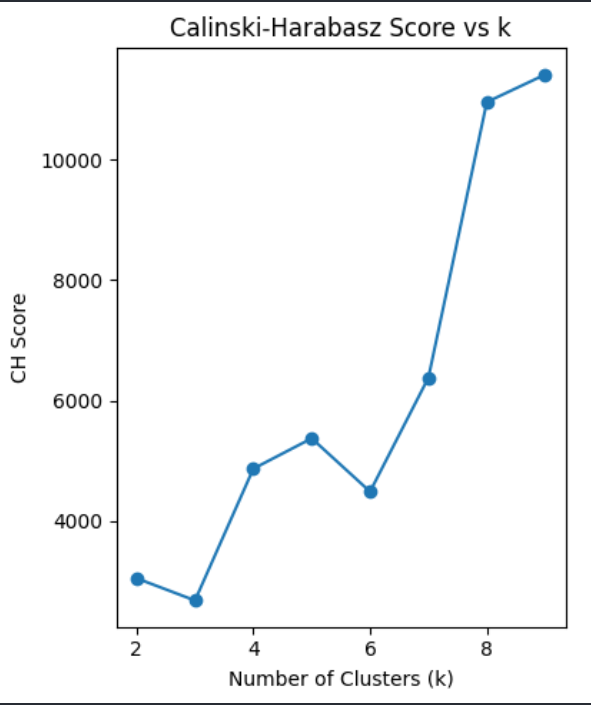
\includegraphics[width=\columnwidth]{calinski-harabasz_score.png}
    \caption{Calinski-Harabasz Scores for Different Values of \(k\)}
    \label{fig:example}
\end{figure}

The Davies-Bouldin Index measures the average similarity between clusters, and is given by:
\begin{equation}
DB = \frac{1}{k} \sum_{i=1}^{k} \max_{j \neq i} \frac{\sigma_i + \sigma_j}{d_{ij}}
\end{equation}

where:
\begin{itemize}
    \item \( \sigma_i \) is the average distance between points in cluster \( i \) and its centroid.
    \item \( \sigma_j \) is the average distance between points in cluster \( j \) and its centroid.
    \item \( d_{ij} \) is the Euclidean distance between cluster centroids \( \mu_i \) and \( \mu_j \).
\end{itemize}

\[ \]

Lower values indicate better clustering and this was observed starting from
where \(k\) was 2. The peak value of Davies-Bouldin index was obtained when
\(k\) was equal to 5, which indicated poor clustering performance.
\begin{figure}[htbp]
    \centering
    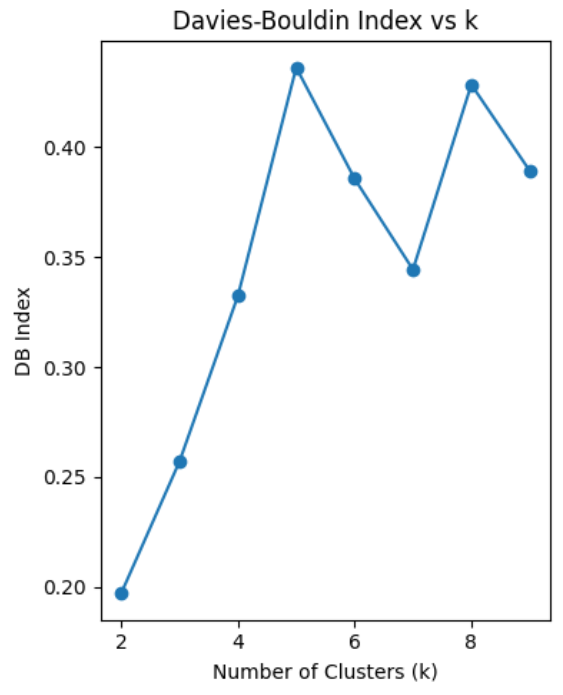
\includegraphics[width=\columnwidth]{davies-bouldin_index.png}
    \caption{Davies-Bouldin Score for Different Values of \(k\)}
    \label{fig:example}
\end{figure}




\begin{figure}[htbp]
    \centering
    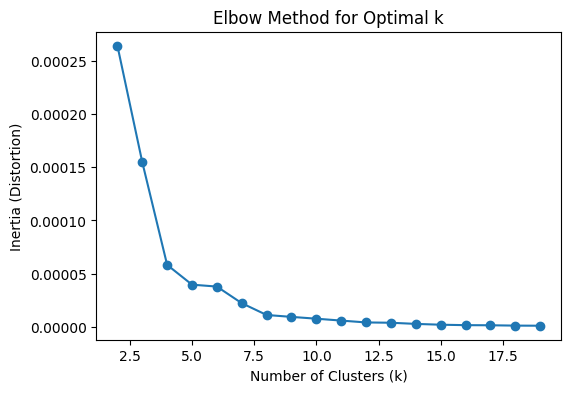
\includegraphics[width=\columnwidth]{elbow_graph.png}
    \caption{Elbow Graph for Different Values of \(k\)}
    \label{fig:example}
\end{figure}



\begin{thebibliography}{00}
\bibitem{b1} W. Li, N. Narvekar, N. Nakshatra, N. Raut, B. Sirkeci and J. Gao,
``Seismic Data Classification Using Machine Learning,'' \textit\{2018 IEEE Fourth
International Conference on Big Data Computing Service and Applications
(BigDataService)\}, Bamberg, Germany, 2018, pp. 56-63 \bibitem{b2} J. Ramirez Jr
and F. G. Meyer, ``Machine Learning for Seismic Signal Processing: Phase
Classification on a Manifold,'' \textit\{2011 10th International Conference on
Machine Learning and Applications and Workshops\}, Honolulu, HI, USA, 2011, pp.
382-388 \bibitem{b3} M. Chakraborty, M. Das and S. Aruchamy, ``Micro-Seismic
Event Detection using statistical feature extraction and machine learning
techniques,'' 2\textit\{022 IEEE 7th International conference for Convergence in
Technology (I2CT)\}, Mumbai, India, 2022, pp. 1-5 \bibitem{b4} H. Shu, A. Y.
Dawod, L. Mu and W. Tepsan, ``A Survey of Machine Learning Applications in
Microseismic Signal Recognition and Classification,'' \textit\{2023 15th
International Conference on Software, Knowledge, Information Management and
Applications (SKIMA)\}, Kuala Lumpur, Malaysia, 2023, pp. 18-23 \bibitem{b5} N.
Varshney, G. Kumar, A. Kumar, S. K. Pandey, T. Singh and K. U. Singh, ``Machine
Learning Based Algorithm for Earthquake Monitoring,'' \textit\{2023 IEEE 12th
International Conference on Communication Systems and Network Technologies
(CSNT)\}, Bhopal, India, 2023, pp. 264-270 \bibitem{b6} T. -L. Chin, C. -Y.
Huang, S. -H. Shen, Y. -C. Tsai, Y. H. Hu and Y. -M. Wu, ``Learn to Detect:
Improving the Accuracy of Earthquake Detection,'' in \textit\{IEEE Transactions on
Geoscience and Remote Sensing\}, vol. 57, no. 11, pp. 8867-8878, Nov. 2019
\bibitem{b7}Y. Shimshoni and N. Intrator, ``Classification of seismic signals by
integrating ensembles of neural networks,'' in \textit\{IEEE Transactions on
Signal Processing\}, vol. 46, no. 5, pp. 1194-1201, May 1998 \bibitem{b8}Agliz,
Driss, and Abderrahman Atmani. ``Seismic signal classification using multi-layer
perceptron neural network.'' \textit\{International Journal of Computer
Applications\} 79, no. 15 (2013). \bibitem{b9}Akhouayri, Es-Saïd, Dris Agliz,
Daniele Zonta, and Abderrahman Atmani. ``A fuzzy expert system for automatic
seismic signal classification.'' \textit{Expert Systems with Applications} 42,
no. 3 (2015): 1013-1027. \bibitem{b10}Curilem, Gloria, Jorge Vergara, Gustavo
Fuentealba, Gonzalo Acuña, and Max Chacón. ``Classification of seismic signals at
Villarrica volcano (Chile) using neural networks and genetic algorithms.''
\textit{Journal of volcanology and geothermal research} 180, no. 1 (2009): 1-8.
\end{thebibliography}
\end{document}
